
\section{Coordenação}
\begin{frame}

\begin{center}
{\huge Capítulo 4 -- Coordenação}
\end{center}

\end{frame}

%-----------------------------------------------------------

\subsection{Abordagens ao Planejamento Multiagente -- SMAs}

\begin{frame}
\frametitle{Abordagens ao Planejamento de SMAs}

\begin{block}{}
 
\begin{itemize}
  \item Coordenação central: controla todos os subplanos
  \item Esquemas de controle distribuído\\
        Conhecimento parcial dos planos de outros agentes
  \item Planejamento Global Negociado

\begin{itemize}
  \item Compartilhamento de todos os planos
  \item Ajuste local para a realização de objetivos comuns

\end{itemize}

\item Modelagem Explícita da Equipe de Agentes
\begin{itemize}
  \item Compromissos conjuntos
   \item Crenças, desejos e intenções comuns

\end{itemize}
\end{itemize}
\end{block}

\end{frame}

%-----------------------------------------------------


\subsection{Exemplos de Coordenação SMAs}

\begin{frame}
\frametitle{Exemplo de Coordenação SMAs}

\begin{figure}[!ht]
\centering
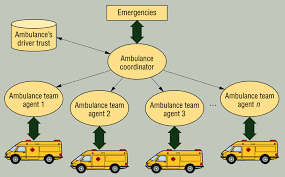
\includegraphics[height =.6\textheight,width=.7\textwidth]{figuras/coordenacao_agentes01.png}
\caption{Coordenação de agentes $\equiv $   SMA}
%\label{ag_01}
\end{figure}
 \end{frame}

%-----------------------------------------------------------

\begin{frame}
\frametitle{Exemplo de Coordenação SMAs}

\begin{figure}[!ht]
\centering
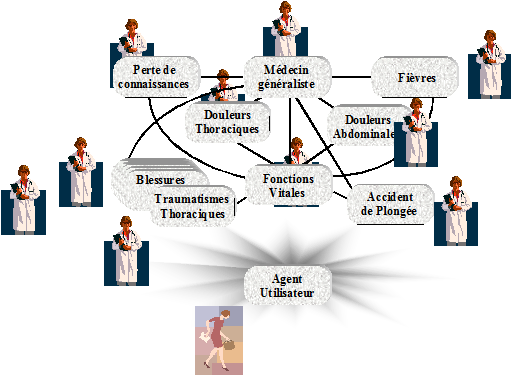
\includegraphics[height =.6\textheight,width=.7\textwidth]{figuras/coordenacao_agentes02.png}
\caption{Coordenação de agentes $\equiv $   SMA}
%\label{ag_01}
\end{figure}
 
\end{frame}

%-----------------------------------------------------------


\section{Estratégias de Jogos}
\begin{frame}

    \frametitle{Teoria de Jogos}
    \begin{itemize}
    \pause
      \item 
\pause
      \item 
    
    \end{itemize}
\end{frame}


%-----------------------------------------------------------



\section{Teoria de Jogos Aplicado a SMA}
\begin{frame}

    \frametitle{Teoria de Jogos Aplicado a SMA}
    \begin{itemize}
    \pause
      \item $\prod^{n}_{x=1} \neq  \prod_{x=1}^{n+1}$
      \item  \url{https://www.codecogs.com/latex/eqneditor.php}
      \item \url{http://www.hostmath.com/}
      

      \pause
      \item 
    
    \end{itemize}
\end{frame}

%-----------------------------------------------------------
